%\begin{appendices}

\appendix
%\chapter*{ANEXOS}% If \appendix doesn't insert a \chapter
%\addcontentsline{toc}{chapter}{ANEXOS}% Print Appendix in ToC
\setcounter{section}{0}% Reset numbering for sections
\renewcommand{\thesection}{\Alph{section}}% Adjust section printing (from here onward)
	
	\section{Árbol de Problemas}
	%\chapter*{Árbol de Problemas}
	%\addcontentsline{toc}{section}{Árbol de Problemas}
	%\renewcommand{\thechapter}{A}
	\label{anexo1}
	\begin{figure}[h]
		\begin{center}
			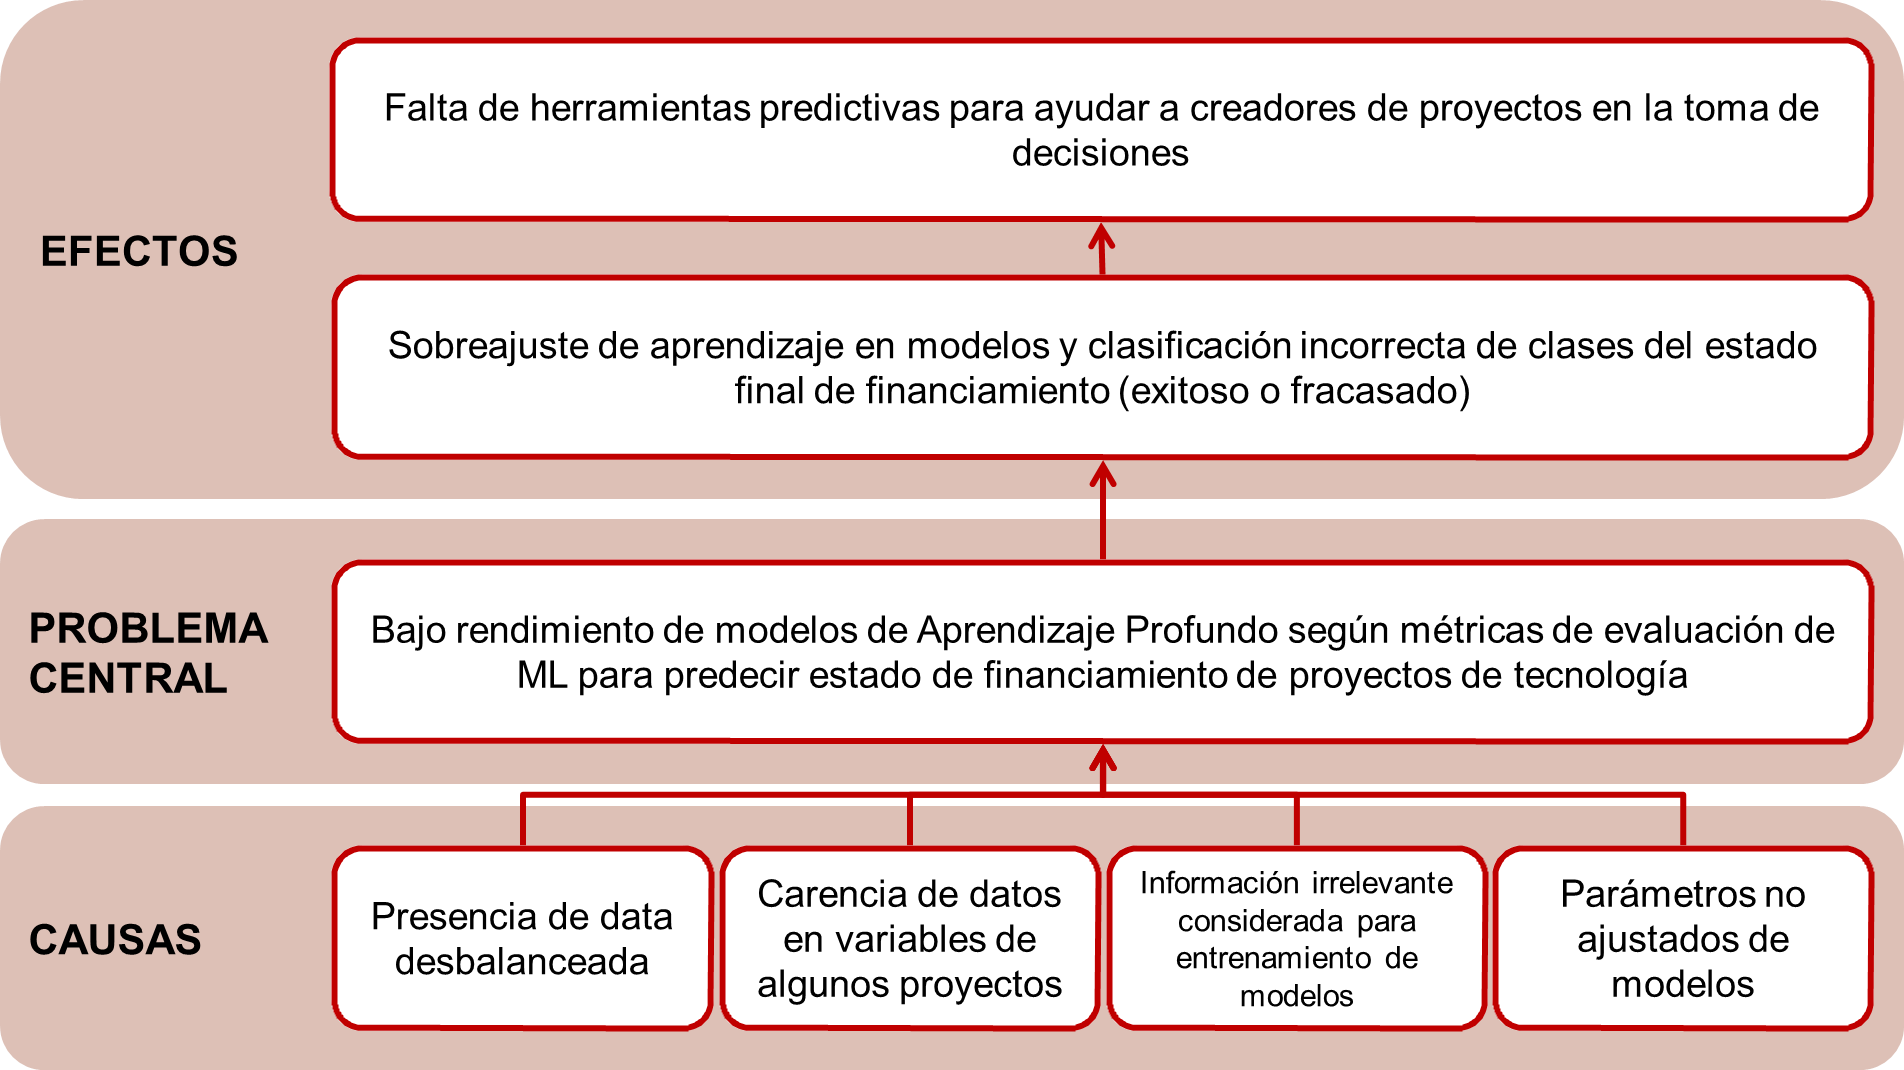
\includegraphics[width=1.05\textwidth]{anexos/arbol_problemas.png}
			%\caption{Fuente: Elaboración propia}
		\end{center}
	\end{figure}
	\clearpage
	
	\section{Árbol de Objetivos}
	%\chapter*{Árbol de Objetivos}
	%\addcontentsline{toc}{section}{Árbol de Objetivos}
	%\renewcommand{\thechapter}{A}
	\label{anexo2}
	\begin{figure}[h]
		\begin{center}
			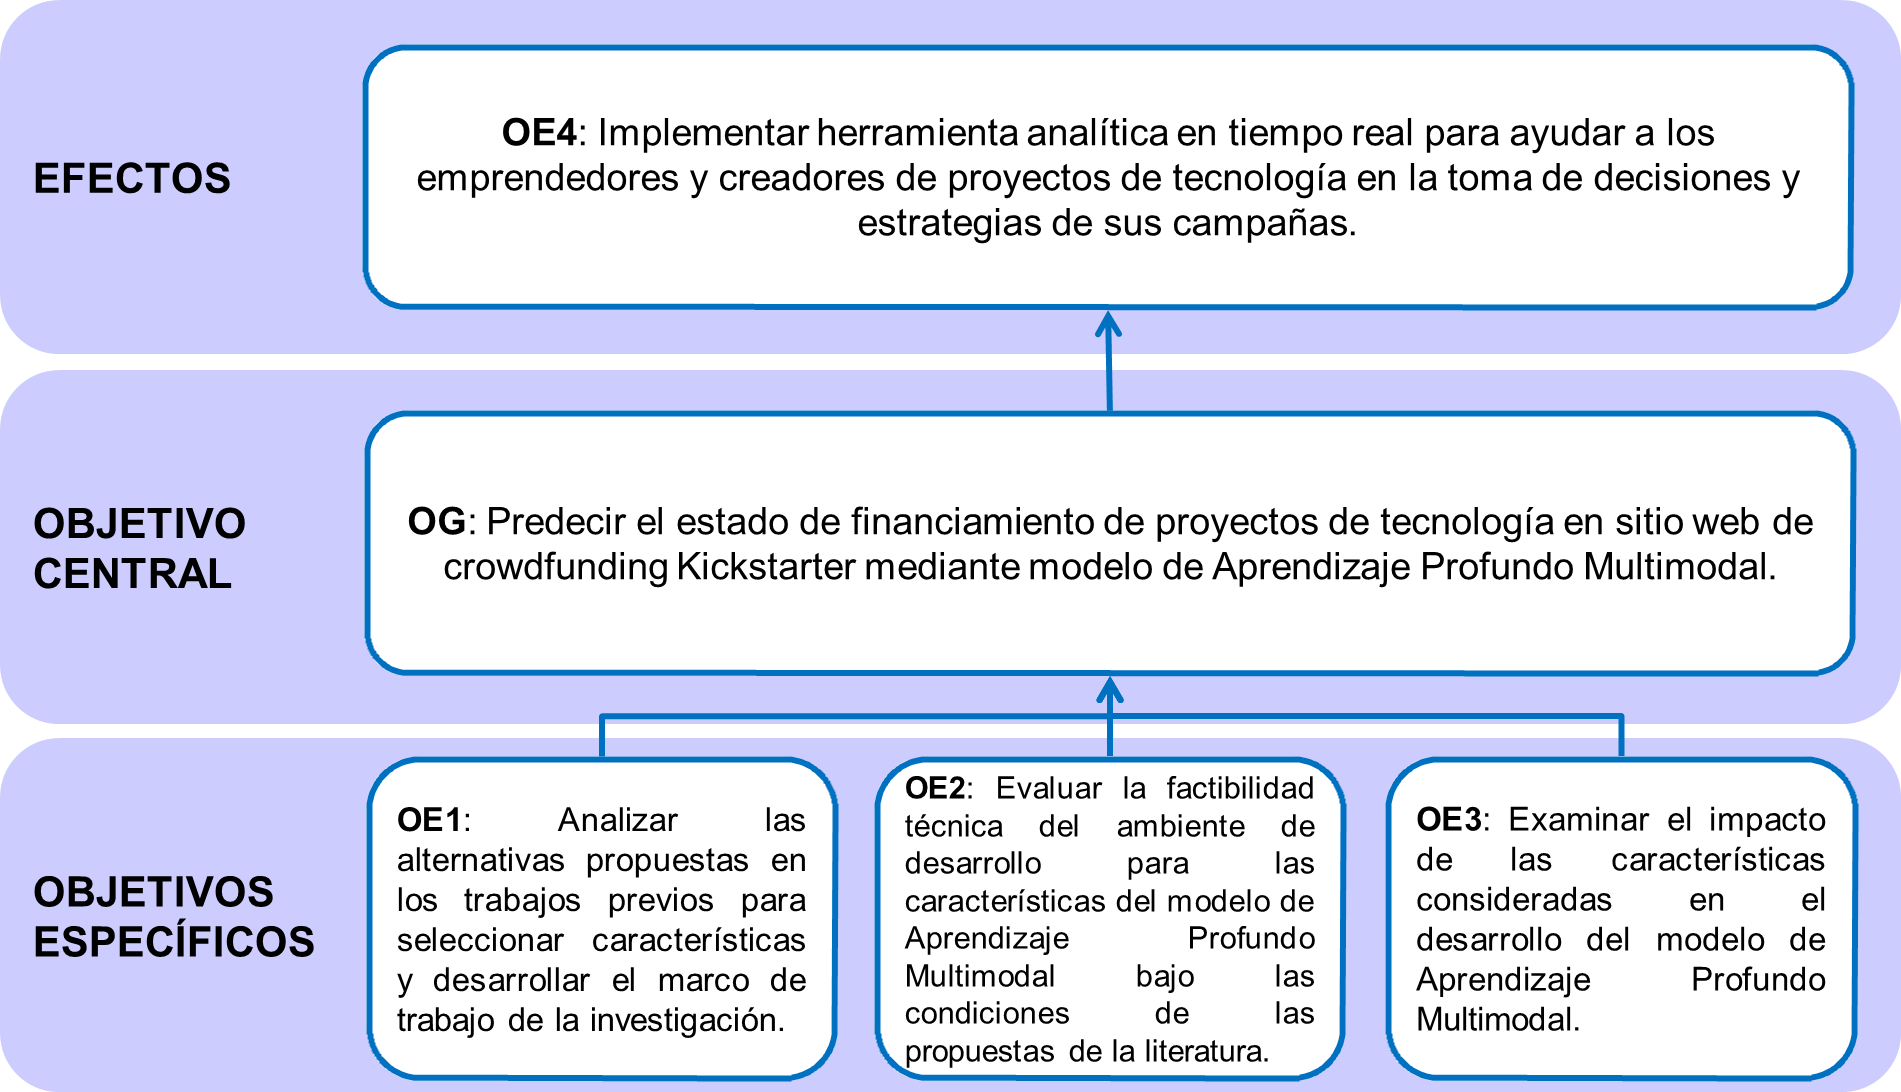
\includegraphics[width=1.05\textwidth]{anexos/arbol_objetivos.png}
			%\caption{Fuente: Elaboración propia}
		\end{center}
	\end{figure}
	\clearpage
	
	\begin{landscape}
		\section{Matriz de Consistencia}
		%\chapter*{Matriz de Consistencia}
		%\addcontentsline{toc}{section}{Matriz de Consistencia}
		%\renewcommand{\thechapter}{A}
		\label{anexo3}
		%\begin{table}[h!]
			\begin{longtable}{ p{5.5cm}p{5.5cm}p{5.5cm}p{5.5cm} }
				%\centering
				\small
				\tabularnewline \specialrule{.1em}{.05em}{.05em}
				\Centering{Problemas}& \Centering{Objetivos}& \Centering{Hipótesis}& \Centering{Variable}\\
				\specialrule{.1em}{.05em}{.05em}
				\Centering{Problema General}& \Centering{Objetivo General} & \Centering{Hipótesis General}& \\
				\hline
				{\ProblemaGeneral} & { \ObjetivoGeneral} & {\HipotesisGeneral} & 
				\setlist{nolistsep}
				\begin{itemize}[label={--},nosep,noitemsep,leftmargin=*,topsep=0pt,partopsep=0pt]
					\item Dependiente: Estado de financiamiento de un proyecto.
					\item Independiente: Modelo de Aprendizaje Profundo Multimodal.
				\end{itemize}
				\\
				\hline
				\Centering{Problemas Específicos}& \Centering{Objetivos Específicos} & \Centering{Hipótesis Específicas} & \\
				\hline
				\vspace{0pt}{\Pbone} & \vspace{0pt}{\Objone} & \vspace{0pt}{\Hone} & 
				\setlist{nolistsep}
				\begin{itemize}[label={--},nosep,noitemsep,leftmargin=*,topsep=0pt,partopsep=0pt]
					\item Dependiente: Estado de financiamiento de un proyecto.
					\item Independiente: Modelo de Aprendizaje Profundo Multimodal.
				\end{itemize}
				\\
				%\hline
				\vspace{0pt}{\Pbtwo} & \vspace{0pt}{\Objtwo} & \vspace{0pt}{\Htwo} & \\
				%\hline
				\vspace{0pt}{\Pbthree} & \vspace{0pt}{\Objthree} & \vspace{0pt}{\Hthree} & \\
				%\hline
				\vspace{0pt}{\Pbfour} & \vspace{0pt}{\Objfour} & \vspace{0pt}{\Hfour} & \\
				\specialrule{.1em}{.05em}{.05em}
			\end{longtable}
			%\caption{Fuente: Elaboración propia}
		%\end{table}
	\end{landscape}
	\clearpage
	
	\section{Comparación de metodologías de antecedentes}
	%\chapter{Comparación de metodologías de antecedentes}
	%\addcontentsline{toc}{section}{Comparación de metodologías de antecedentes}
	\label{anexo4}
	%\begin{table}[htbp]
	\begingroup
		\renewcommand\arraystretch{0.5}
		\begin{longtable}{M{3cm}M{5.5cm}M{5.5cm}M{1.5cm}}
			\centering
			\small
			%% Se agrega tabularnewline para longtable
			\tabularnewline \specialrule{.1em}{.05em}{.05em}
			Autor & Título de la Investigación & Metodología & Grupo
			\\
			\specialrule{.1em}{.05em}{.05em}
			Chen, Jones, Kim \& Schlamp
			& KickPredict: Predicting Kickstarter Success
			& \setlist{nolistsep}
			\begin{itemize}[label={--},nosep,noitemsep,leftmargin=*,topsep=0pt,partopsep=0pt]
				\item Recolección de datos.
				\item Modelamiento.
				\item Evaluación.
				\item Despliegue.
			\end{itemize}
			& GG
			\\
			\hline
			Mitra \& Gilbert
			& The Language that Gets People to Give: Phrases that Predict Success on Kickstarter
			& \setlist{nolistsep}
			\begin{itemize}[label={--},nosep,noitemsep,leftmargin=*,topsep=0pt,partopsep=0pt]
				\item Recolección de datos.
				\item Pre-procesamiento de datos.
				\item Modelamiento.
				\item Evaluación.
				\item Despliegue.
			\end{itemize}
			& GE
			\\
			\hline
			Zhou, Zhang, Wang, Du, Qiao \& Fan
			& Money Talks: A Predictive Model on Crowdfunding Success Using Project Description
			& \setlist{nolistsep}
			\begin{itemize}[label={--},nosep,noitemsep,leftmargin=*,topsep=0pt,partopsep=0pt]
				\item Formulación del problema.
				\item Recolección de datos.
				\item Pre-procesamiento de datos.
				\item Modemiento.
				\item Evaluación.
			\end{itemize}
			& GD
			\\
			\hline
			Chen, Chen, Chen, Yang, Lin \& Wei
			& Will Your Project Get the Green Light? Predicting the Success of Crowdfunding Campaigns
			& \setlist{nolistsep}
			\begin{itemize}[label={--},nosep,noitemsep,leftmargin=*,topsep=0pt,partopsep=0pt]
				\item Recolección de datos.
				\item Pre-procesamiento de datos.
				\item Modelamiento.
				\item Evaluación.
			\end{itemize}
			& GF
			\\
			\hline
			Beckwith
			& Predicting Success in Equity Crowdfunding
			& \setlist{nolistsep}
			\begin{itemize}[label={--},nosep,noitemsep,leftmargin=*,topsep=0pt,partopsep=0pt]
				\item Recolección de datos.
				\item Pre-procesamiento de datos.
				\item Modelamiento.
				\item Evaluación.
			\end{itemize}
			&  GF
			\\
			\hline
			Li, Rakesh \& Reddy
			& Project Success Prediction in Crowdfunding Environments
			& \setlist{nolistsep}
			\begin{itemize}[label={--},nosep,noitemsep,leftmargin=*,topsep=0pt,partopsep=0pt]
				\item Formulación del problema.
				\item Recolección de datos.
				\item Pre-procesamiento de datos.
				\item Modelamiento.
				\item Evaluación.
			\end{itemize}
			& GD
			\\
			\hline
			Yuan, Lau \& Xu
			& The Determinants of Crowdfunding Success: A Semantic Text Analytics Approach
			& \setlist{nolistsep}
			\begin{itemize}[label={--},nosep,noitemsep,leftmargin=*,topsep=0pt,partopsep=0pt]
				\item Recolección de datos.
				\item Pre-procesamiento de datos.
				\item Modelamiento.
				\item Evaluación.
				\item Despliegue.
			\end{itemize}
			& GE
			\\
			\hline
			Sawhney, Tran \& Tuason
			& Using Language to Predict Kickstarter Success
			& \setlist{nolistsep}
			\begin{itemize}[label={--},nosep,noitemsep,leftmargin=*,topsep=0pt,partopsep=0pt]
				\item Recolección de datos.
				\item Modelamiento.
				\item Evaluación.
			\end{itemize}
			& GH
			\\
			\hline
			Kaur \& Gera
			& Effect of Social Media Connectivity on Success of Crowdfunding Campaigns
			& \setlist{nolistsep}
			\begin{itemize}[label={--},nosep,noitemsep,leftmargin=*,topsep=0pt,partopsep=0pt]
				\item Recolección de datos.
				\item Pre-procesamiento de datos.
				\item Modelamiento.
				\item Evaluación.
			\end{itemize}
			& GF
			\\
			\hline
			Kamath \& Kamat
			& Supervised Learning Model For Kickstarter Campaigns With R Mining
			& \setlist{nolistsep}
			\begin{itemize}[label={--},nosep,noitemsep,leftmargin=*,topsep=0pt,partopsep=0pt]
				\item Formulación del problema.
				\item Recolección y pre-procesamiento de datos.
				\item Exploración y extracción de datos.
				\item Modelamiento.
				\item Evaluación.
			\end{itemize}
			& GD
			\\
			\hline
			Yu, Huang, Yang, Liu, Li \& Tsai
			& Prediction of Crowdfunding Project Success with Deep Learning
			& \setlist{nolistsep}
			\begin{itemize}[label={--},nosep,noitemsep,leftmargin=*,topsep=0pt,partopsep=0pt]
				\item Recolección de datos.
				\item Exploración de datos.
				\item Pre-procesamiento de datos.
				\item Modelamiento.
				\item Evaluación.
			\end{itemize}
			& GE
			\\
			\hline
			Lee, Lee \& Kim
			& Content-based Success Prediction of Crowdfunding Campaigns: A Deep Learning Approach
			& \setlist{nolistsep}
			\begin{itemize}[label={--},nosep,noitemsep,leftmargin=*,topsep=0pt,partopsep=0pt]
				\item Recolección de datos.
				\item Modelamiento.
				\item Evaluación.
			\end{itemize}
			& GH
			\\
			\hline
			Jin, Zhao, Chen, Liu \& Ge
			& Estimating the Days to Success of Campaigns in Crowdfunding: A Deep Survival Perspective
			& \setlist{nolistsep}
			\begin{itemize}[label={--},nosep,noitemsep,leftmargin=*,topsep=0pt,partopsep=0pt]
				\item Formulación del problema.
				\item Recolección de datos.
				\item Pre-procesamiento de datos.
				\item Modelamiento.
				\item Evaluación.
				\item Despliegue.
			\end{itemize}
			& GA
			\\
			\hline
			Cheng, Tan, Hou \& Wei
			& Success Prediction on Crowdfunding with Multimodal Deep Learning
			& \setlist{nolistsep}
			\begin{itemize}[label={--},nosep,noitemsep,leftmargin=*,topsep=0pt,partopsep=0pt]
				\item Formulación del problema.
				\item Recolección de datos.
				\item Pre-procesamiento de datos.
				\item Modelamiento.
				\item Evaluación.
				\item Despliegue.
			\end{itemize}
			& GA
			\\
			\hline
			Chen \& Shen
			& Finding the Keywords Affecting the Success of Crowdfunding Projects
			& \setlist{nolistsep}
			\begin{itemize}[label={--},nosep,noitemsep,leftmargin=*,topsep=0pt,partopsep=0pt]
				\item Recolección de datos.
				\item Pre-procesamiento de datos.
				\item Selección de características.
				\item Modelamiento.
				\item Evaluación.
			\end{itemize}
			& GC
			\\
			\hline
			Chaichi \& Anderson
			& Deploying Natural Language Processing to Extract Key Product Features of Crowdfunding Campaigns: The Case of 3D Printing Technologies on Kickstarter
			& \setlist{nolistsep}
			\begin{itemize}[label={--},nosep,noitemsep,leftmargin=*,topsep=0pt,partopsep=0pt]
				\item Recolección de datos.
				\item Pre-procesamiento de datos.
				\item Selección de características.
				\item Modelamiento.
				\item Evaluación.
			\end{itemize}
			& GC
			\\
			\hline
			Shafqat \& Byun
			& Topic Predictions and Optimized Recommendation Mechanism Based on Integrated Topic Modeling and Deep Neural Networks in Crowdfunding Platforms
			& \setlist{nolistsep}
			\begin{itemize}[label={--},nosep,noitemsep,leftmargin=*,topsep=0pt,partopsep=0pt]
				\item Formulación del problema.
				\item Recolección de datos.
				\item Selección de características.
				\item Modelamiento.
				\item Evaluación.
				\item Despliegue.
			\end{itemize}
			& GB
			\\
			\hline
			Fernández-Blanco, Villanueva-Balsera, Rodriguez-Montequin \& Moran-Palacios
			& Key Factors for Project Crowdfunding Success: An Empirical Study
			& \setlist{nolistsep}
			\begin{itemize}[label={--},nosep,noitemsep,leftmargin=*,topsep=0pt,partopsep=0pt]
				\item Entendimiento del problema.
				\item Entendimiento de los datos.
				\item Preparación de los datos.
				\item Modelamiento.
				\item Evaluación.
				\item Despliegue.
			\end{itemize}
			& CRISP-DM
			\\
			\specialrule{.1em}{.05em}{.05em}
		\end{longtable}%
	\endgroup
	%\end{table}
	\clearpage
	
	\begin{landscape}
		\section{Comparación de objetivos específicos de antecedentes}
		\label{anexo5}
	\end{landscape}
	
	\clearpage
	
	\section{Parámetros para modelo predictivo de Metainformación}
	\label{anexo6}
	%\begin{table}[h!]
	%\begingroup
		%\renewcommand\arraystretch{0.5}
		\begin{longtable}{ m{8cm}m{7cm} }
			\centering
			\small
			\tabularnewline \specialrule{.1em}{.05em}{.05em}
			\Centering{Hiperparámetro}& \Centering{Valor}\\
			\specialrule{.1em}{.05em}{.05em}
			\vspace{0pt}Pesos de clases & \setlist{nolistsep}
			\begin{minipage}[t]{\linewidth}
			\begin{itemize}[label={--},noitemsep,leftmargin=*,nosep,after=\strut]
				\item Exitoso (1): $1.7581290322580645$
				\item Fracasado (0): $0.6987077585764833$
			\end{itemize}
			\end{minipage}
			\\
			%\hline
			Optimizador & \setlist{nolistsep}
			\begin{minipage}[t]{\linewidth}
			\begin{itemize}[label={--},noitemsep,leftmargin=*,nosep,after=\strut]
				\item Nombre: ADAM
				\item Ratio de aprendizaje: $5*10^{-3}$
				\item Ratio de decaimiento: $1*10^{-5}$
			\end{itemize}
			\end{minipage}
			\\
			%\hline
			Parada temprana & \setlist{nolistsep}
			\begin{minipage}[t]{\linewidth}
			\begin{itemize}[label={--},noitemsep,leftmargin=*,nosep,after=\strut]
				\item Monitor: \textit{val\_accuracy}
				\item Modo: \textit{auto}
				\item Paciencia: 10
			\end{itemize}
			\end{minipage}
			\\
			%\hline
			Reducción de ratio de aprendizaje & \setlist{nolistsep}
			\begin{minipage}[t]{\linewidth}
			\begin{itemize}[label={--},noitemsep,leftmargin=*,nosep,after=\strut]
				\item Monitor: \textit{val\_accuracy}
				\item Modo: \textit{max}
				\item Paciencia: 3
				\item Factor: 0.1
			\end{itemize}
			\end{minipage}
			\\
			%\hline
			Punto de guardado del modelo & \setlist{nolistsep}
			\begin{minipage}[t]{\linewidth}
				\begin{itemize}[label={--},noitemsep,leftmargin=*,nosep,after=\strut]
					\item Monitor: \textit{val\_loss}
					\item Modo: \textit{min}
				\end{itemize}
			\end{minipage}
			\\
			%\hline
			Función de pérdida & \textit{binary\_crossentropy}
			\\
			%\hline
			Número de épocas & 100
			\\
			%\hline
			Tamaño de lote & 128
			\\
			%\hline
			Datos de entrada & \textit{X\_train}
			\\
			%\hline
			Datos de destino & \textit{y\_train}
			\\
			%\hline
			Datos de validación & \textit{X\_test}, \hspace{5mm} \textit{y\_test}
			\\
			\hline
			\vspace{0pt}Longitud de datos de entrada - capa de entrada & \vspace{0pt}6
			\\
			%\hline
			\vspace{0pt}Número de neuronas de salida - capa densa 1 & \vspace{0pt}32
			\\
			%\hline
			\vspace{0pt}Función de activación - capa densa 1 & \vspace{0pt}\textit{relu}
			\\
			%\hline
			\vspace{0pt}Ratio de capa de desactivación 1 & \vspace{0pt}0.25
			\\
			%\hline
			\vspace{0pt}Número de neuronas de salida - capa densa 2 & \vspace{0pt}16
			\\
			%\hline
			\vspace{0pt}Función de activación - capa densa 2 & \vspace{0pt}\textit{tanh}
			\\
			%\hline
			\vspace{0pt}Ratio de capa de desactivación 2 & \vspace{0pt}0.30
			\\
			%\hline
			\vspace{0pt}Función de activación - capa final & \vspace{0pt}\textit{sigmoid}
			\\
			\specialrule{.1em}{.05em}{.05em}
		\end{longtable}
	%\end{table}
	%\endgroup	
	\clearpage
	
	\section{Parámetros para modelo predictivo de Descripción}
	\label{anexo7}
	%\begin{table}[h!]
	%\begingroup
	%\renewcommand\arraystretch{0.5}
	\begin{longtable}{ m{8cm}m{7cm} }
		\centering
		\small
		\tabularnewline \specialrule{.1em}{.05em}{.05em}
		\Centering{Hiperparámetro}& \Centering{Valor}\\
		\specialrule{.1em}{.05em}{.05em}
		\vspace{0pt}Pesos de clases & \setlist{nolistsep}
		\begin{minipage}[t]{\linewidth}
			\begin{itemize}[label={--},noitemsep,leftmargin=*,nosep,after=\strut]
				\item Exitoso (1): $1.7581290322580645$
				\item Fracasado (0): $0.6987077585764833$
			\end{itemize}
		\end{minipage}
		\\
		%\hline
		Optimizador & \setlist{nolistsep}
		\begin{minipage}[t]{\linewidth}
			\begin{itemize}[label={--},noitemsep,leftmargin=*,nosep,after=\strut]
				\item Nombre: ADAM
				\item Ratio de aprendizaje: $1*10^{-5}$
				\item Ratio de decaimiento: $1*10^{-5}$
			\end{itemize}
		\end{minipage}
		\\
		%\hline
		Parada temprana & \setlist{nolistsep}
		\begin{minipage}[t]{\linewidth}
			\begin{itemize}[label={--},noitemsep,leftmargin=*,nosep,after=\strut]
				\item Monitor: \textit{val\_loss}
				\item Modo: \textit{min}
				\item Paciencia: 10
			\end{itemize}
		\end{minipage}
		\\
		%\hline
		Reducción de ratio de aprendizaje & \setlist{nolistsep}
		\begin{minipage}[t]{\linewidth}
			\begin{itemize}[label={--},noitemsep,leftmargin=*,nosep,after=\strut]
				\item Monitor: \textit{val\_accuracy}
				\item Modo: \textit{max}
				\item Paciencia: 5
				\item Factor: 0.01
			\end{itemize}
		\end{minipage}
		\\
		%\hline
		Punto de guardado del modelo & \setlist{nolistsep}
		\begin{minipage}[t]{\linewidth}
			\begin{itemize}[label={--},noitemsep,leftmargin=*,nosep,after=\strut]
				\item Monitor: \textit{val\_loss}
				\item Modo: \textit{min}
			\end{itemize}
		\end{minipage}
		\\
		%\hline
		Función de pérdida & \textit{binary\_crossentropy}
		\\
		%\hline
		Número de épocas & 100
		\\
		%\hline
		Tamaño de lote & 128
		\\
		%\hline
		Datos de entrada & \textit{training\_sentences}
		\\
		%\hline
		Datos de destino & \textit{training\_labels}
		\\
		%\hline
		Datos de validación & \textit{testing\_sentences}, \hspace{5mm} \textit{testing\_labels}
		\\
		\hline
		\vspace{0pt}Longitud de datos de entrada - capa de entrada & \vspace{0pt}3,671
		\\
		%\hline
		\vspace{0pt}Tamaño de vocabulario - capa Embedding & \vspace{0pt}148,270
		\\
		%\hline
		\vspace{0pt}Dimensión de incrustación - capa Embedding & \vspace{0pt}100
		\\
		%\hline
		\vspace{0pt}Número de filtros - capa Conv1D & \vspace{0pt}128
		\\
		%\hline
		\vspace{0pt}Tamaño de kernel - capa Conv1D & \vspace{0pt}5
		\\
		%\hline
		\vspace{0pt}Número de neuronas de salida - capa densa 1 & \vspace{0pt}64
		\\
		%\hline
		\vspace{0pt}Función de activación - capa densa 1 & \vspace{0pt}tanh
		\\
		%\hline
		\vspace{0pt}Función de activación - capa final & \vspace{0pt}\textit{sigmoid}
		\\
		\specialrule{.1em}{.05em}{.05em}
	\end{longtable}
	%\end{table}
	%\endgroup
	\clearpage
	
	\section{Parámetros para modelo predictivo de Comentarios}
	\label{anexo8}
	%\begin{table}[h!]
	%\begingroup
	%\renewcommand\arraystretch{0.5}
	\begin{longtable}{ m{8cm}m{7cm} }
		\centering
		\small
		\tabularnewline \specialrule{.1em}{.05em}{.05em}
		\Centering{Hiperparámetro}& \Centering{Valor}\\
		\specialrule{.1em}{.05em}{.05em}
		\vspace{0pt}Pesos de clases & \setlist{nolistsep}
		\begin{minipage}[t]{\linewidth}
			\begin{itemize}[label={--},noitemsep,leftmargin=*,nosep,after=\strut]
				\item Exitoso (1): $1.7581290322580645$
				\item Fracasado (0): $0.6987077585764833$
			\end{itemize}
		\end{minipage}
		\\
		%\hline
		Optimizador & \setlist{nolistsep}
		\begin{minipage}[t]{\linewidth}
			\begin{itemize}[label={--},noitemsep,leftmargin=*,nosep,after=\strut]
				\item Nombre: ADAM
				\item Ratio de aprendizaje: $1*10^{-3}$
				\item Ratio de decaimiento: $1*10^{-6}$
			\end{itemize}
		\end{minipage}
		\\
		%\hline
		Parada temprana & \setlist{nolistsep}
		\begin{minipage}[t]{\linewidth}
			\begin{itemize}[label={--},noitemsep,leftmargin=*,nosep,after=\strut]
				\item Monitor: \textit{val\_loss}
				\item Modo: \textit{min}
				\item Paciencia: 10
			\end{itemize}
		\end{minipage}
		\\
		%\hline
		Reducción de ratio de aprendizaje & \setlist{nolistsep}
		\begin{minipage}[t]{\linewidth}
			\begin{itemize}[label={--},noitemsep,leftmargin=*,nosep,after=\strut]
				\item Monitor: \textit{val\_accuracy}
				\item Modo: \textit{max}
				\item Paciencia: 5
				\item Factor: 0.01
			\end{itemize}
		\end{minipage}
		\\
		%\hline
		Punto de guardado del modelo & \setlist{nolistsep}
		\begin{minipage}[t]{\linewidth}
			\begin{itemize}[label={--},noitemsep,leftmargin=*,nosep,after=\strut]
				\item Monitor: \textit{val\_loss}
				\item Modo: \textit{min}
			\end{itemize}
		\end{minipage}
		\\
		%\hline
		Función de pérdida & \textit{binary\_crossentropy}
		\\
		%\hline
		Número de épocas & 50
		\\
		%\hline
		Tamaño de lote & 64
		\\
		%\hline
		Datos de entrada & \textit{training\_sentences}
		\\
		%\hline
		Datos de destino & \textit{training\_labels}
		\\
		%\hline
		Datos de validación & \textit{testing\_sentences}, \hspace{5mm} \textit{testing\_labels}
		\\
		\hline
		\vspace{0pt}Longitud de datos de entrada - capa de entrada & \vspace{0pt}5,000
		\\
		%\hline
		\vspace{0pt}Tamaño de vocabulario - capa Embedding & \vspace{0pt}74,096
		\\
		%\hline
		\vspace{0pt}Dimensión de incrustación - capa Embedding & \vspace{0pt}100
		\\
		%\hline
		\vspace{0pt}Ratio de capa de desactivación & \vspace{0pt}0.50
		\\
		%\hline
		\vspace{0pt}Número de neuronas de salida - capa Bidireccional LSTM & \vspace{0pt}128
		\\
		%\hline
		\vspace{0pt}Función de activación - capa final & \vspace{0pt}\textit{sigmoid}
		\\
		\specialrule{.1em}{.05em}{.05em}
	\end{longtable}
	%\end{table}
	%\endgroup
	\clearpage
	
	\section{Parámetros para modelo de Aprendizaje Profundo Multimodal}
	\label{anexo9}
	%\begin{table}[h!]
	%\begingroup
	%\renewcommand\arraystretch{0.5}
	\begin{longtable}{ m{8.7cm}m{7cm} }
		\centering
		\small
		\tabularnewline \specialrule{.1em}{.05em}{.05em}
		\Centering{Hiperparámetro}& \Centering{Valor}\\
		\specialrule{.1em}{.05em}{.05em}
		\vspace{0pt}Pesos de clases & \setlist{nolistsep}
		\begin{minipage}[t]{\linewidth}
			\begin{itemize}[label={--},noitemsep,leftmargin=*,nosep,after=\strut]
				\item Exitoso (1): $1.7581290322580645$
				\item Fracasado (0): $0.6987077585764833$
			\end{itemize}
		\end{minipage}
		\\
		%\hline
		Optimizador & \setlist{nolistsep}
		\begin{minipage}[t]{\linewidth}
			\begin{itemize}[label={--},noitemsep,leftmargin=*,nosep,after=\strut]
				\item Nombre: ADAM
				\item Ratio de aprendizaje: $1*10^{-5}$
				\item Ratio de decaimiento: $1*10^{-5}$
			\end{itemize}
		\end{minipage}
		\\
		%\hline
		Parada temprana & \setlist{nolistsep}
		\begin{minipage}[t]{\linewidth}
			\begin{itemize}[label={--},noitemsep,leftmargin=*,nosep,after=\strut]
				\item Monitor: \textit{val\_loss}
				\item Modo: \textit{min}
				\item Paciencia: 10
			\end{itemize}
		\end{minipage}
		\\
		%\hline
		Reducción de ratio de aprendizaje & \setlist{nolistsep}
		\begin{minipage}[t]{\linewidth}
			\begin{itemize}[label={--},noitemsep,leftmargin=*,nosep,after=\strut]
				\item Monitor: \textit{val\_accuracy}
				\item Modo: \textit{max}
				\item Paciencia: 5
				\item Factor: 0.01
			\end{itemize}
		\end{minipage}
		\\
		%\hline
		Punto de guardado del modelo & \setlist{nolistsep}
		\begin{minipage}[t]{\linewidth}
			\begin{itemize}[label={--},noitemsep,leftmargin=*,nosep,after=\strut]
				\item Monitor: \textit{val\_loss}
				\item Modo: \textit{min}
			\end{itemize}
		\end{minipage}
		\\
		%\hline
		Función de pérdida & \textit{binary\_crossentropy}
		\\
		%\hline
		Número de épocas & 200
		\\
		%\hline
		Tamaño de lote & 32$^a$
		\\
		%\hline
		Datos de entrada & \textit{X\_train\_stacked}$^b$
		\\
		%\hline
		Datos de destino & \textit{y\_train}
		\\
		%\hline
		Datos de validación & \textit{X\_test\_stacked}$^c$, \hspace{5mm} \textit{y\_test}
		\\
		\hline
		%\hline
		\vspace{0pt}Longitud de datos de entrada$^d$ & \vspace{0pt}3,671, \hspace{5mm}5,000, \hspace{5mm}6
		\\
		%\hline
		\vspace{0pt}Número de neuronas de entrada - capa concatenada$^e$ & \vspace{0pt}1, \hspace{5mm}1, \hspace{5mm}1
		\\
		%\hline
		\vspace{0pt}Número de neuronas de salida - capa concatenada & \vspace{0pt}3
		\\
		%\hline
		\vspace{0pt}Número de neuronas de salida - capa densa 1 & \vspace{0pt}10
		\\
		%\hline
		\vspace{0pt}Función de activación - capa densa 1 & \vspace{0pt}\textit{relu}
		\\
		%\hline
		\vspace{0pt}Función de activación - capa final & \vspace{0pt}\textit{sigmoid}
		\\
		\specialrule{.1em}{.05em}{.05em}
	\end{longtable}
	\begin{flushleft}
		\footnotesize{$^a$ Al no especificarse, por defecto se asignó el valor de 32 \parencite{tec_keras_modeltraining}; $^b$ comprende la concatenación de \textit{X\_train\_description}, \textit{X\_train\_comments} y \textit{X\_train\_metadata}; $^c$ comprende la concatenación de \textit{X\_test\_description}, \textit{X\_test\_comments} y \textit{X\_test\_metadata}; $^d$ representan las longitudes de datos de entrada de cada modalidad; $^e$ representan las salidas de cada modalidad}
	\end{flushleft}
	%\end{table}
	%\endgroup
	\clearpage
%\end{appendices} 